%!TEX TS-program = xelatex
\documentclass[12pt, a4paper]{article}  

\usepackage{etex} % расширение классического tex в частности позволяет подгружать гораздо больше пакетов, чем мы и займёмся далее

%%%%%%%%%% Математика %%%%%%%%%%
\usepackage{amsmath,amsfonts,amssymb,amsthm,mathtools} 
%\mathtoolsset{showonlyrefs=true}  % Показывать номера только у тех формул, на которые есть \eqref{} в тексте.
%\usepackage{leqno} % Нумерация формул слева


%%%%%%%%%%%%%%%%%%%%%%%% Шрифты %%%%%%%%%%%%%%%%%%%%%%%%%%%%%%%%%
\usepackage{fontspec}         % пакет для подгрузки шрифтов
\setmainfont{Arial}   % задаёт основной шрифт документа

\defaultfontfeatures{Mapping=tex-text}

% why do we need \newfontfamily:
% http://tex.stackexchange.com/questions/91507/
\newfontfamily{\cyrillicfonttt}{Arial}
\newfontfamily{\cyrillicfont}{Arial}
\newfontfamily{\cyrillicfontsf}{Arial}

\usepackage{unicode-math}     % пакет для установки математического шрифта
\setmathfont{Asana-Math.otf}      % шрифт для математики
% \setmathfont[math-style=ISO]{Asana Math}
% Можно делать смену начертания с помощью разных стилей

% Конкретный символ из конкретного шрифта
% \setmathfont[range=\int]{Neo Euler}

\usepackage{polyglossia}      % Пакет, который позволяет подгружать русские буквы
\setdefaultlanguage{russian}  % Основной язык документа
\setotherlanguage{english}    % Второстепенный язык документа


%%%%%%%%%% Работа с картинками %%%%%%%%%
\usepackage{graphicx}                  % Для вставки рисунков
\usepackage{graphics}
\graphicspath{{Pictures/}}    % можно указать папки с картинками
\usepackage{wrapfig}                   % Обтекание рисунков и таблиц текстом


%%%%%%%%%% Работа с таблицами %%%%%%%%%%
\usepackage{tabularx}            % новые типы колонок
\usepackage{tabulary}            % и ещё новые типы колонок
\usepackage{array}               % Дополнительная работа с таблицами
\usepackage{longtable}           % Длинные таблицы
\usepackage{multirow}            % Слияние строк в таблице
\usepackage{float}               % возможность позиционировать объекты в нужном месте
\usepackage{booktabs}            % таблицы как в книгах!
\renewcommand{\arraystretch}{1.3} % больше расстояние между строками

% Заповеди из документации к booktabs:
% 1. Будь проще! Глазам должно быть комфортно
% 2. Не используйте вертикальные линни
% 3. Не используйте двойные линии. Как правило, достаточно трёх горизонтальных линий
% 4. Единицы измерения - в шапку таблицы
% 5. Не сокращайте .1 вместо 0.1
% 6. Повторяющееся значение повторяйте, а не говорите "то же"
% 7. Есть сомнения? Выравнивай по левому краю!





%%%%%%%%%% Графика и рисование %%%%%%%%%%
\usepackage{tikz, pgfplots}  % язык для рисования графики из latex'a
\usepackage{amscd}                  %Пакеты для рисования
\usepackage[matrix,arrow,curve]{xy} %комунитативных диаграмм





%%%%%%%%%% Свои команды %%%%%%%%%%
\usepackage{etoolbox}    % логические операторы для своих макросов
\usepackage{xparse}      % больше команд для создания команд
\DeclareMathOperator{\Var}{Var}
\DeclareMathOperator{\Cov}{Cov}
\renewcommand{\labelitemi}{\color[named]{blue}{$\bullet$}}
\usepackage{etoolbox}
% Все свои команды лучше всего определять не по ходу текста, как это сделано в этом документе, а в преамбуле!


% Пакет, который ставит в каждом первом абзаце главы красную строку
% Просто, чтобы эта pdf-ка нормально смотрелась :)
\usepackage{indentfirst}  
\setkeys{russian}{babelshorthands=true}
% обо всех волшебных строках на следующем семинаре! 
\pgfplotsset {compat = 1.13}
\begin{document}
\section{Первое задание}
\subsection{}
\renewcommand{\theequation}{Eq.(\arabic{equation})}
В пространстве случайных величин с конечным вторым моментом 
$L^2(\Omega,\;\mathcal{F},\;\mathbb{P})$ неравенство Коши --- Буняковского имеет вид:\\
\begin{equation}
\Cov^2(X,Y)\leq\Var[X]\cdot\Var[Y]
\end{equation}
\subsection{}
\newcommand{\s}{\ensuremath{\sigma}}
\s-алгебра --- алгебра множеств, замкнутая относительно операции счётного объединения. \s-алгебры играют важнейшую роль в~теории меры и~интегралов Лебега, а~также в~теории вероятностей.
\subsection{}
\newcommand{\X}{\ensuremath{x_1 \ldots x_n}}
Пусть \X --- выборка из распределения вероятности. Тогда выборочная дисперсия --- это случайная величина вида:\\
\begin{equation}
S_n^2=\frac{1}{n}\cdot\sum_{i=1}^{n}(X_i-\bar{X})^2
\end{equation}
\subsection{}
\newcommand{\com}[2]{\ensuremath{x_{#1}\ldots x_{#2}}}
\begin{itemize}
\item \com{a}{z}\\
\item \com{1}{6}\\
\item \com{(a,b)}{(c,d)}
\end{itemize}
\subsection{}
\begin{itemize}
\item Первый пункт
\item Второй пункт
\item Третий пункт
\end{itemize}
\subsection{}
\newcommand{\llim}{\lim\limits}
\begin{equation}
\llim_{x \to 0} \frac{\sin{x}}{x} = 1
\end{equation}
\subsection{}
\renewcommand{\thefigure}{\arabic{section}:\arabic{figure}}
\begin{figure}[H] 
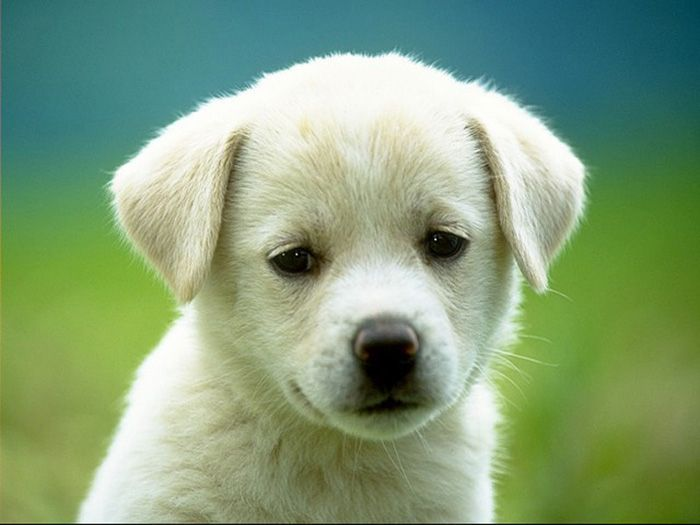
\includegraphics[scale=0.5]{1.jpg}
\caption{Грустный песик}
\end{figure}
\subsection{}
\begin{equation}
D=\frac{\rho_b}{\rho_{bs}}\cdot100
\end{equation}
\end{document}